% !TeX spellcheck = en_US

\chapter{Evaluation}
\section{Evaluation on Datasets}
\label{sec:EvaluationOnDatasets} % Now, we can use "\autoref{sec:<my-label>}" to refer to this chapter
The face segmentation network was tested on two different datasets with real-life images: 1.) The Caltech occluded faces in the wild (COFW) by \cite{cofw} and 2.) parts-labeled LFW Dataset of the University of Massachusetts \cite{LFW_dataset}. Both datasets are designed to present faces in real-world conditions. The COFW dataset provides 29 landmarks and a bounding box for all 507 images. The original LFW dataset contains 13'000 images of 1'680 different subjects. Each face is labeled with the name of the subject. This database is actually meant to test facial recognition/verification algorithms on it. Nevertheless, we tested the segmentation of the FCN on the 500 image parts-LFW validation set. For each image there is a ground truth segmentation, which makes it possible to measure the quality of the FCN's segmentation in numbers.
\\
\subsection{COFW}
Since on the COFW dataset, only landmarks and bounding-boxes are given, the segmentation had to be evaluated qualitatively. We were't able to count the correctly labeled pixels of the FCN with respect to a ground-truth mask. To increase the precision of the network, we cropped the images according to the given bounding-boxes. Because the bounding-boxes were only including the eyes and the mouth of the subject, we had to add an offset which was determined by eye. Nevertheless, we tried to reconstruct the graphic on Nirkis \cite{nirkin2018_faceswap} github-repository 'face\_segmentation' (Figure \ref{fig:chap2:myMatrix}). In the next Figure (Figure \ref{fig:chap2:myMatrix_EGGER}) the same 18 images are segmented by the iterative method of Egger et al. This algorithm outputs both, a model and a segmentation. In Figure \ref{fig:chap2:COFW_Fits} are the fits of 9 images with both masks (segmentations) used. A matrix of the other 9 fits can be found in the Appendix.

\begin{figure}[h]
	\centering
	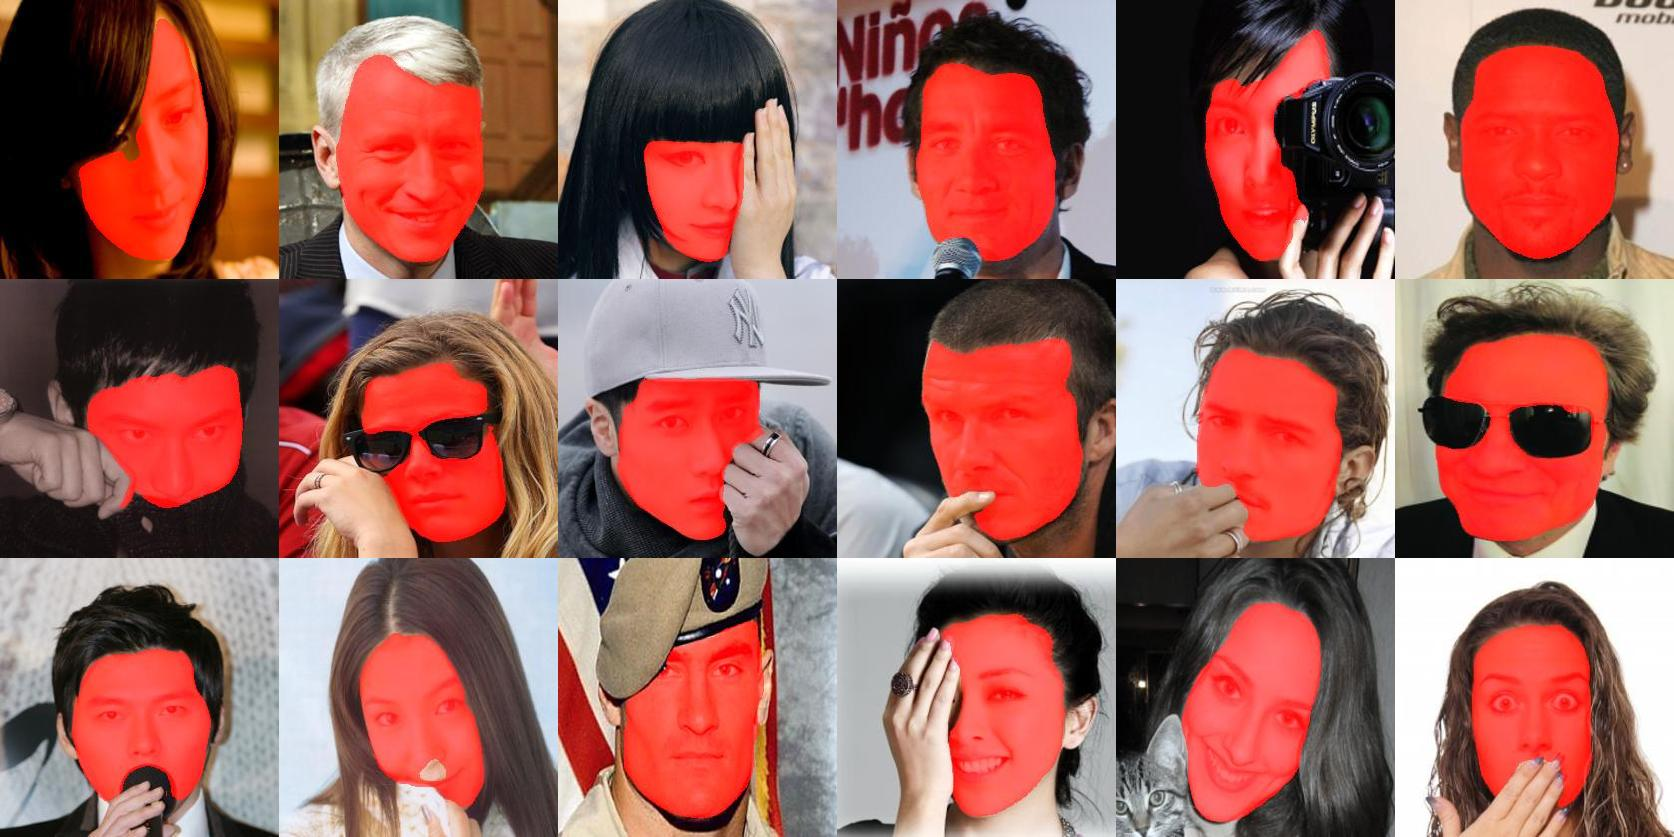
\includegraphics[width=0.9\textwidth]{Figures/chap2/myMatrix.jpg}
	\caption{18 images of the COFW Dataset overlayd with the FCN output (in red). The segmentation results are very similar to those on \href{https://github.com/YuvalNirkin/face_segmentation}{Nirkin's github page}.}
	\label{fig:chap2:myMatrix}
\end{figure}

\begin{figure}[h]
	\centering
	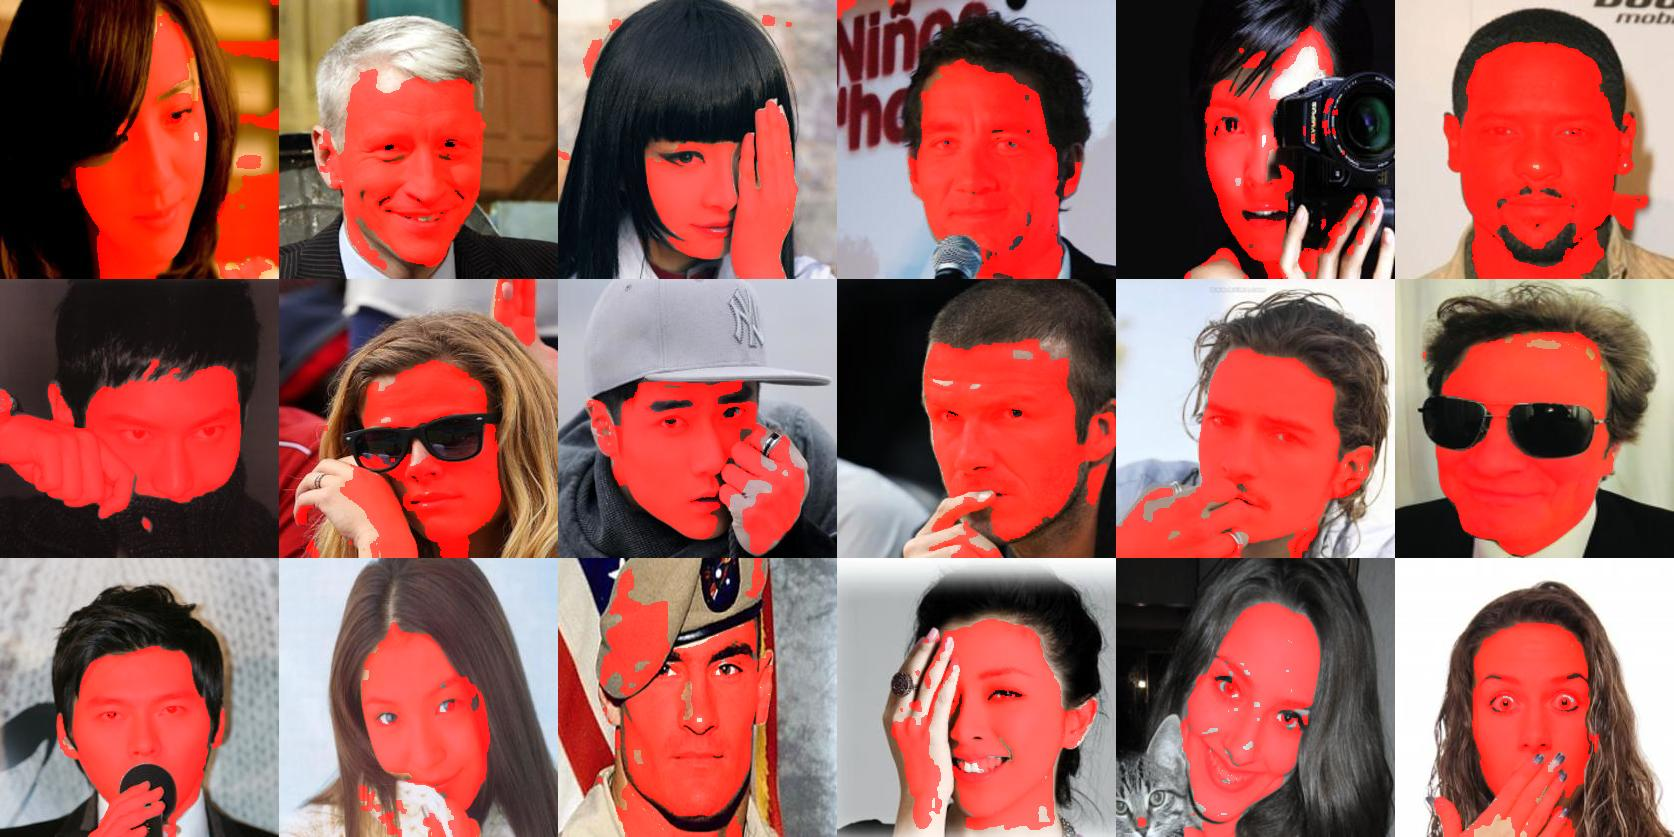
\includegraphics[width=0.9\textwidth]{Figures/chap2/myMatrix_EGGER.jpg}
	\caption{Exactly the same images as in Figure \ref{fig:chap2:myMatrix}, but this time with the (final) segmentation of the occlusion-aware method of Egger et al. \cite{egger_paper}. Often the eyes are not segmented or the segmentation includes skin other than the face (eg. hands).}
	\label{fig:chap2:myMatrix_EGGER}
\end{figure}

\begin{figure}[h]
	\centering
	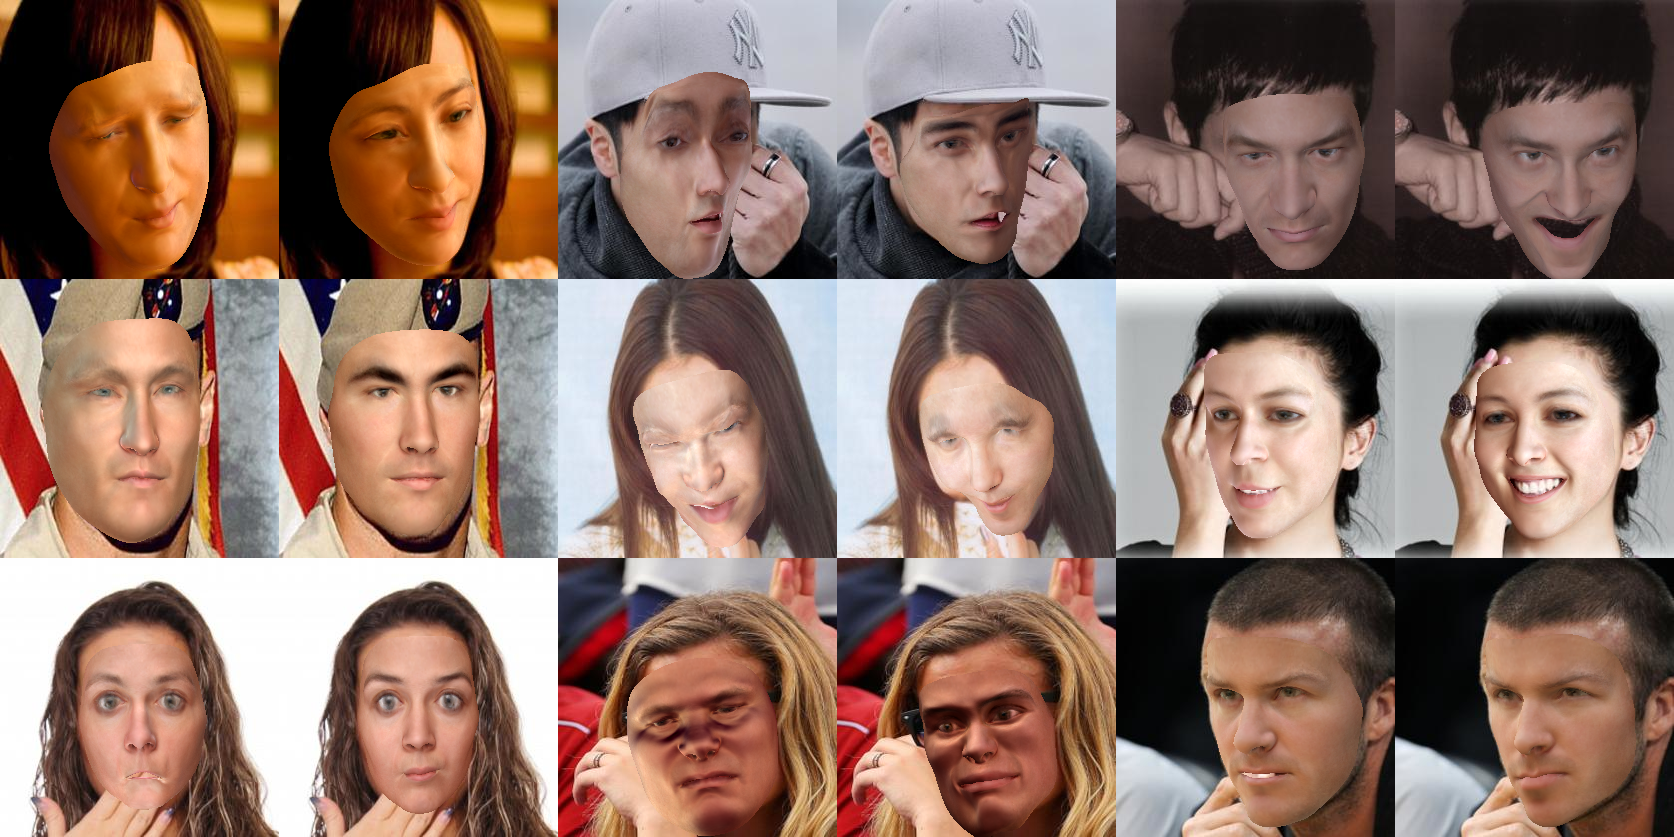
\includegraphics[width=0.9\textwidth]{Figures/chap2/COFW_Fits.png}
	\caption{Tuples of facial images. In every tuple, the first image shows the fit with the mask of the algorithm of Egger et al. itself (Figure \ref{fig:chap2:myMatrix_EGGER}). The second shows the fit with the FCN mask which are depicted in Figure \ref{fig:chap2:myMatrix}.}
	\label{fig:chap2:COFW_Fits}
\end{figure}


\begin{figure}
	\centering
	\subbottom[An facial-image with the segmentation of the FCN highlited in red]{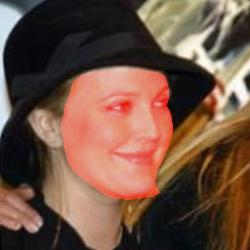
\includegraphics[width=0.4\textwidth]{Figures/chap2/drew/drew_original.jpg}\label{fig:drew:sf1}}
	\subbottom[The provided ground-truth segmentation of the image \ref{fig:drew:sf1} overlaid with the mask of the FCN (red)]{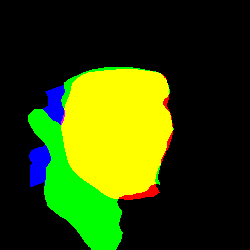
\includegraphics[width=0.4\textwidth]{Figures/chap2/drew/drew_segments.png}\label{fig:drew:sf2}}
	
	
	\subbottom[An facial-image with the segmentation of the FCN highlited in red]{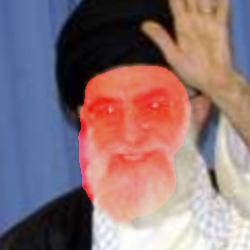
\includegraphics[width=0.4\textwidth]{Figures/chap2/ali/ali_original.jpg}\label{fig:ali:sf3}}
	\subbottom[The provided ground-truth segmentation of the image \ref{fig:ali:sf3} overlaid with the mask of the FCN (red)]{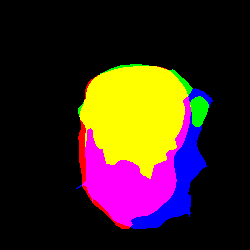
\includegraphics[width=0.4\textwidth]{Figures/chap2/ali/ali_segments.png}\label{fig:ali:sf4}}
	\caption{Plots of four Turing machines}
	\label{fig:tm}
\end{figure}

\subsection{Parts-LFW}
In the Parts-LFW dataset, we had a ground-truth mask for every image. The mask distinguishes between hair, skin and background. We looped trough all the provided ground-truth masks and overlaid them with the segmentations of the FCN. Now, we can compare the labels of both masks. The evaluation is quite impressive. The FCN performs very good in segmenting only pixels which belong to the face. In average over the 500 images of the Parts LFW dataset, there are $98.5\%$ right non-segmentations (only 1.5\% False Positives). On the other hand, only $85.4\%$ of all the pixels which belong to the face are segmented as face (4.6\% False Negatives) which is not a good but acceptable result. Figures \ref{fig:drew:sf1} and \ref{fig:drew:sf2} depict such a face image and it's mask. Unfortunately, on the given mask, no distinction is made between face and other parts of the body, but everything is segmented as skin (Sub-figures \ref{fig:drew:sf1} and \ref{fig:drew:sf2}). However, more problematic is that some faces have beards. The FCN of \cite{nirkin2018_faceswap} segmented facial hair which was excluded on the provided labels. So we had to manually remove these images (Sub-figures \ref{fig:ali:sf3} and \ref{fig:ali:sf4}). To reduce the effort, we took the Parts-LFW validation set containing 500 images. After removing the ones with a beard or mustache, we were left with 447 images. The results are summarized in Figure \ref{fig:Parts-LFW}.

\begin{figure}
\begin{center}
\begin{tabular}{l|l} \hline
	false-positives (hair) & 7.04\%\\ \hline
	false-positives (background) & 0.68\%\\ \hline
	right-segmentations & 85.87\%\\ \hline
	right non-sementations & 99.32\% \\ \hline
\end{tabular}
\end{center}
\caption{The averages over the 447 images of the Parts-LFW evaluation set of \cite{LFW_dataset}. The FCN recognizes (almost) only pixels, which belong to the face (little false positives). By reducing from 500 to 447 images, we were able to reduce them. Unfortunately, there are many false negatives (skin pixels labeled as background).} 
\label{fig:Parts-LFW}
\end{figure}
%\vspace{.5cm}

\section{Evaluation on Synthetic-Data}
In order to evaluate the FCN on synthetic-data, we used the Parametric-Face-Image-Generator of \cite{parametric} to produce images of a random face in a given pose (see  \Cref{fig:syntheticData_samples}). We extended the software so that it now renders occlusions over the face. Further, we changed the Parametric-Face-Image-Generator so it now generates a Ground-Truth-Mask, which classifies every pixel either as part of the face or as non-face.\\
\\
Nirkin et al. \cite{nirkin2018_faceswap} claim that both the face itself an the context of the face play an important role for the outcome of the segmentation. To measure this effect and reduce the impact of outliers, we repeat each experiment multiple times with a different face and a different background image. All images we use for the following tests were generated with the same illumination. Each experiment with the synthetic face images is based on the average outcome of 10 datasets with different subjects.

\begin{figure}[h]
	\centering
	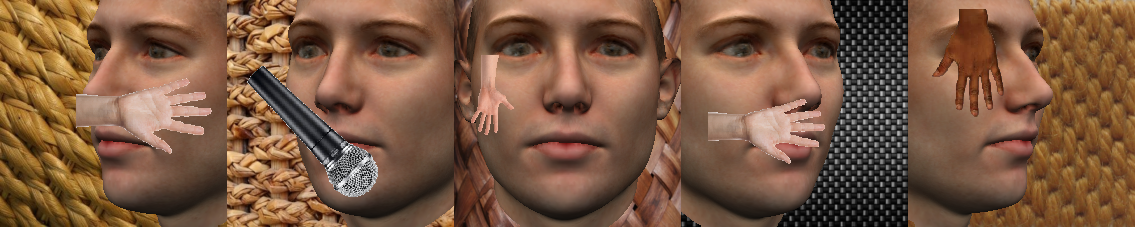
\includegraphics[width=\textwidth]{Figures/chap2/syntheticData_samples.png}
	\caption{Five examples of the synthetic face images. The same face is shown with yaw angles $-45$\textdegree, $-25$\textdegree, $0$\textdegree, $25$\textdegree, and $45$\textdegree. The occlusion is randomly choosen and in a random orientation and position.}
	\label{fig:syntheticData_samples}
\end{figure}

\subsection{Dependence of the Euler angles}
Because we can now create synthetic face images in any desired pose, we first wanted to find out the accuracy of segmenting the FCN for the angles: Yaw, Roll, and Pitch. In order to do that, we produced with the tool of \cite{parametric} 101 face images for every integer angle from $-50$\textdegree to $50$\textdegree. In every picture, the face is turned one degree further. We evaluated each angle itself and every possible combination of the angles in order to create a hierarchy under the angles (results in \Cref{fig:evaluation_angles}).\\
\\
From the graphs of \Cref{fig:evaluation_angles} we can conclude that the roll angle is the most relevant for the FCN, that the pitch-angle is less important and that the accuracy of the FCN is still good even with high yaw angles (least important). 

\begin{figure}[h]
	\centering
	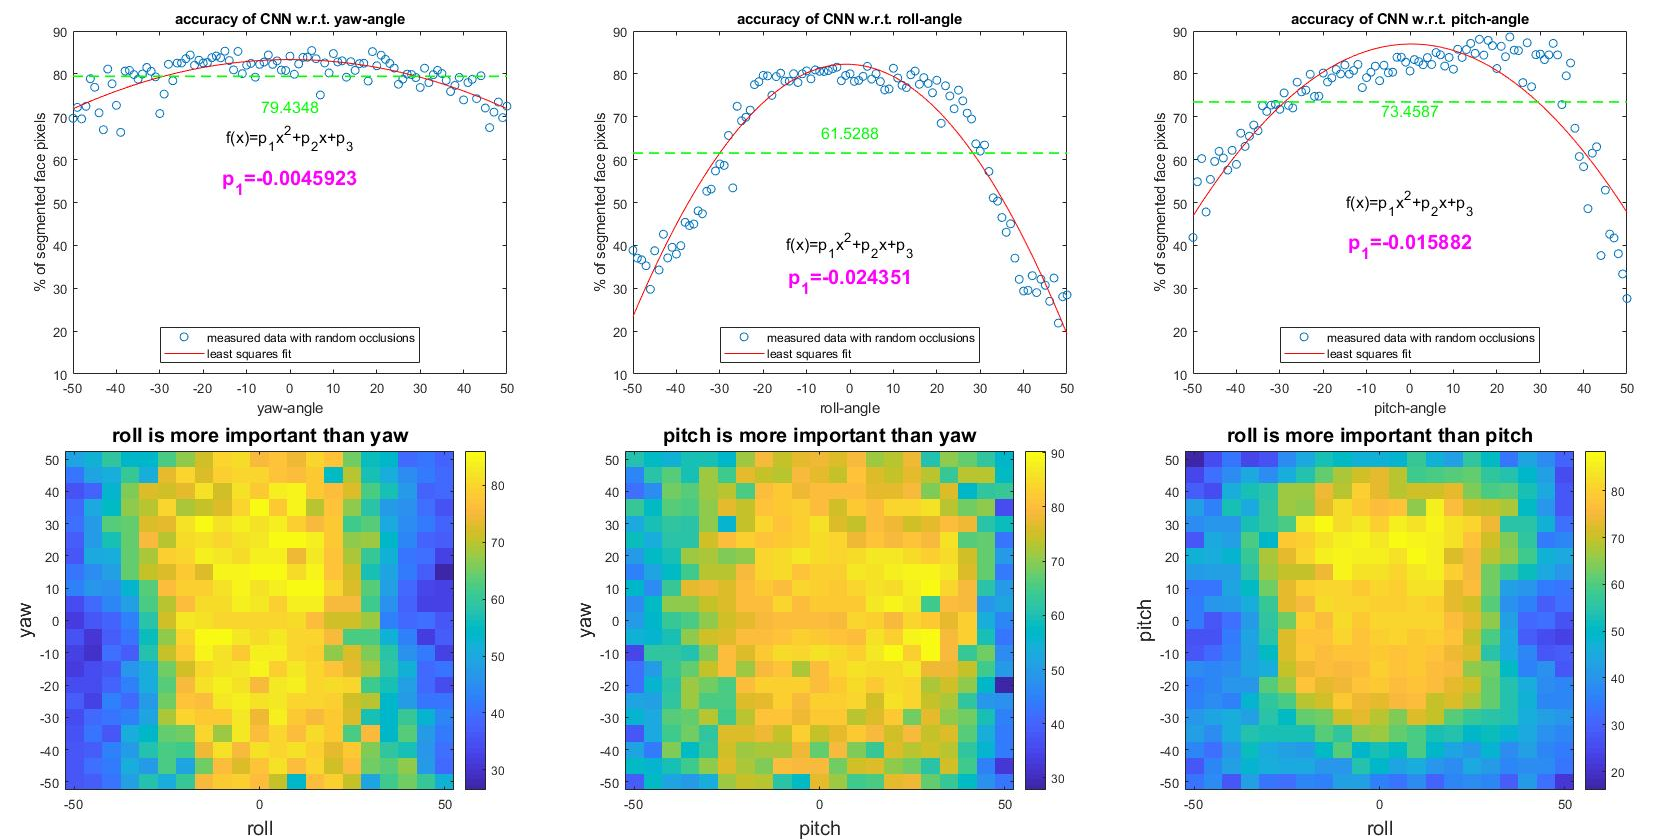
\includegraphics[width=\textwidth]{Figures/evaluation_angles.png}
	\caption{In the plots on the top row we see the segmetation accuracy in percent (on the y-axis) for every single image (with face angle from $-50$\textdegree to $50$\textdegree on the x-axis). The point cloud is approximated by a quadratic function via a least squares fit (red curve / $f(x)$). The first parameter of this function determines the opening angle ($p_1$). In the bottom row the colors indicate the segmentation accuracy. The brighter the color, the better the segmentation. In every plot, there is a cluster of high accuracy segmentations centered in the origin. The angle on whose axis the cluster has the smaller extent is the more important of the two. We call an angle 'important', when a small change of this angle leads to a failure of the FCN.}
	\label{fig:evaluation_angles}
\end{figure}

\subsection{random boxes as occlusions}
With the parametric-face-image-generator of \cite{parametric}, we produced about 5.2 thousand images splitted up in three datasets. Every dataset contains images for 20 occlusion levels, where one angle is in the range from $-40$\textdegree to $40$\textdegree and the other two angles are set to $0$. To reduce the impact of one individual face, each dataset is reproduced 5 times with a different face. The results are in \Cref{fig:occVal40} and \Cref{fig:occVal90}\\
\\
In the given table of \Cref{fig:angle_table}, all provided images show a face, from which 20\% of the pixels are occluded by a randomly colored box. We can optically verify, that 1) the yaw-angle, despite the occluding box, has not much of an effect. 2.) In both situations, $-40$\textdegree and $40$\textdegree, of the roll angle, the result is not satisfying. That's interesting, because no matter how big the roll-angle is, the information (the face) stays the same. 3.) In the third column, the segmentation with a negative pitch angle is much worse than with a positive one! This supports our assumption that the roll-angle plays a big role, followed by the (asymmetric) pitch-angle. The yaw-angle is less important because even at large angles much of the face is still segmented.\\

% The source for this table was this post: https://stackoverflow.com/questions/2771856/centering-text-horizontally-and-vertically-in-latex
% To add padding for the cell contents: https://tex.stackexchange.com/questions/31672/column-and-row-padding-in-tables
\begin{figure}[h]
	\begin{center}
		\newcolumntype{C}{>{\centering\arraybackslash} m{2cm} }  %# New column type
		\begin{tabular}{m{1cm}|SC|SC|SC}
			& yaw & roll & pitch\\ \hline
			-40 & \subfloat{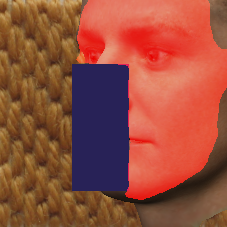
\includegraphics[width=0.1\textwidth]{Figures/-40_0_0_occVal_20.png}} &
			\subfloat{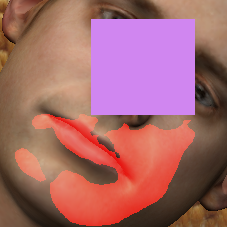
\includegraphics[width=0.1\textwidth]{Figures/0_0_-40_occVal_20.png}} &
			\subfloat{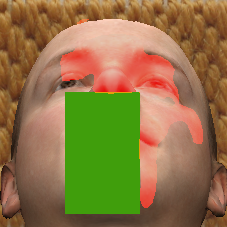
\includegraphics[width=0.1\textwidth]{Figures/0_-40_0_occVal_20.png}} \\ \hline
			40 & \subfloat{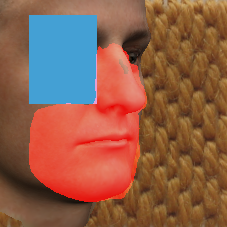
\includegraphics[width=0.1\textwidth]{Figures/40_0_0_occVal_20.png}} &
			\subfloat{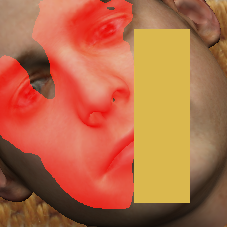
\includegraphics[width=0.1\textwidth]{Figures/0_0_40_occVal_20.png}} &
			\subfloat{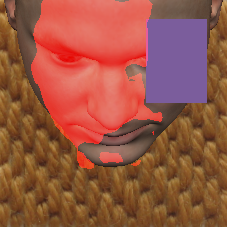
\includegraphics[width=0.1\textwidth]{Figures/0_40_0_occVal_20.png}} \\
		\end{tabular}
	\end{center}
	\caption{Based on these images, we can see that the roll angle (rotation) is the most sensitive, followed by the pitch angle (tilt), where the segmentation works better on positive angles than on negative ones. The most stable detection is at the yaw angle. It has the least influence on the segmentation.}
	\label{fig:angle_table}
\end{figure}
Although boxes as occlusions are very simple and we're in control of the rectangle's size, we can occlude a given amount of the face region with this method, but in practice, exact rectangles are very rare. That's why we left it with the rectangles and used real-world objects (e.g. hands, microphones or sunglasses) as synthetic occlusions. Unlike Nirkin[1], we didn't use the landmarks of the face for this task. We placed them randomly on the image instead. Thats the reason why we use a second plot to show the percentage of occluded face pixels in the following.

\begin{figure}
	\centering
	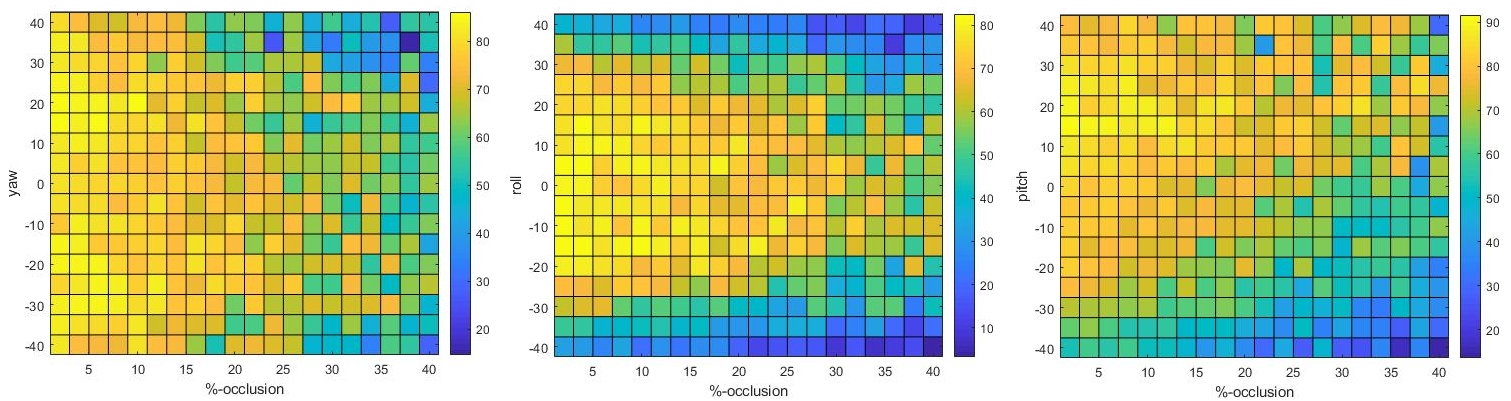
\includegraphics[width=\textwidth]{Figures/occVal_angles.png}
	\caption{The color of each grid cell indicates the accuracy of the segmentation of the FCN on a set of faces turned by the corresponding angle and occluded with a square, so that the corresponding amount (on the x-axis) of the face is hidden. The brighter the color, the better the segmentation. On each plot, we would expect to see a triangle pointing to the right. This means that the combination of a large angle and a large occlusion make the face even more unsegmentable.}
	\label{fig:occVal40}
\end{figure}

We see that the segmentation is very sensitive to roll-angles and the FCN is not trained to segment faces in every rotation! Surprisingly, the yaw angle plays a subordinate role here. The right most plot of \Cref{fig:occVal90} tells us, that the sign of the pitch angle plays a significant role! Since we aren't able to determine at which angles exactly the FCN begins to fail,we repeated the experiment with a higher angle range:\\

\begin{figure}[b]
	\centering
	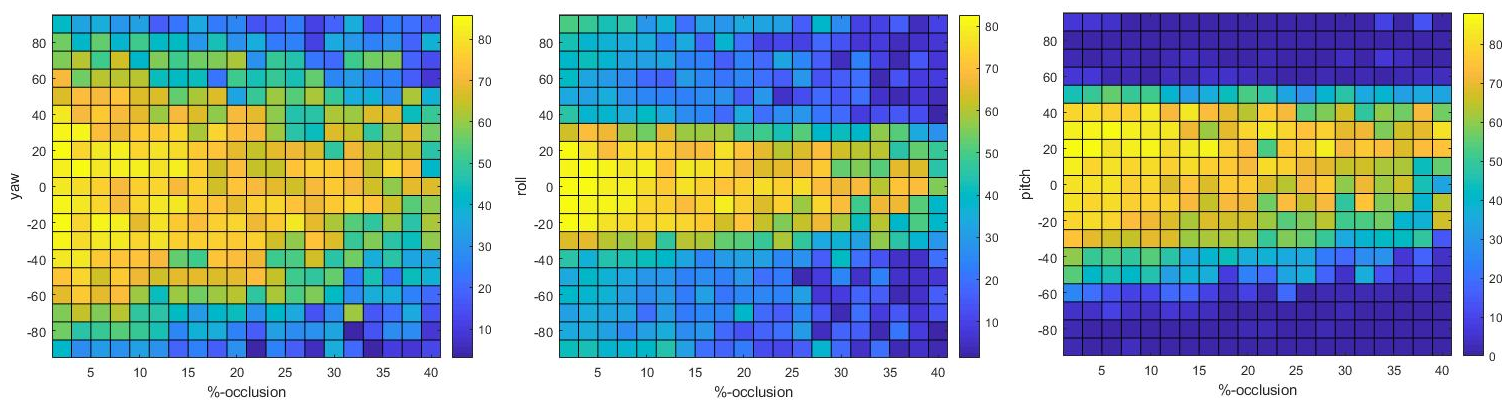
\includegraphics[width=\textwidth]{Figures/occVal_angles_90.png}
	\caption{This plot shows the outcome of a similar expreiment as snown in Figure \ref{fig:occVal40} with less resolution. All the angles (yaw, pitch and roll) range from $-90$\textdegree to $90$ \textdegree. The scale on the "\%-occlusion" stays the same as in Figure \ref{fig:occVal40} We can clearly see the limits of the FCN even with a occlusion of 2\%! Very interesting is the hard transition from good segmentations to bad segmentations in the two right plots.}
	\label{fig:occVal90}
\end{figure}

\FloatBarrier

\section{Parametric-Face-Image-Generator}
As metioned at the beginning of this chapter, we extended the Parametric-Face-Image-Generator of \cite{parametric}. In our version the option "occlusionMode" in the configuration files can now be set to:
\begin{itemize}
	\item \textbf{"eyes"}: A circle occludes the picture centered on the pupil centers of the face.
	\item \textbf{"random-1"}: A  hand hides the picture in a random place in a random orientation.
	\item \textbf{"random-2"}: A  microphone hides the picture in a random place in a random orientation.
	\item \textbf{"random"}: A randomly chosen occlusion image hides the picture in a random place.
	\item \textbf{"box"}: Boxes, filled with an arbitrary color hides the image.
	\item \textbf{"box-whiteNoise"}: Boxes, filled with Gaussian white noise hides the image.
	\item \textbf{"box-skinColor"}: Boxes, filled with the color at the tip of the chin hide the image in a random place.
	\item \textbf{"box-[0-100]"}: Boxes, filled with a random color sized that they occlude the specified amount of face pixels.
	\item \textbf{"loop"}: Produces 20 copies of the same image, each wit a box occluding 2,4,6,...,40 \% of the face.
	\item \textbf{"texture"}: Fulls a randomly placed box with a texture image specified in the folder 'testures'.
\end{itemize}
The software provides csv-Files, rps-Files, tlms-Files, ground truth masks, images with occlusions and images without occlusions for both the 'bfm' version and for the tailored 'face12' version of the Basel Face Model. If an occlusion gets rendered over a landmark, it gets disabled, which was of use in the next chapter (see Figure \ref{fig:chap3:lms}).